

\documentclass[twocolumn,12pt,journal]{IEEEtran_modified}
\usepackage{graphicx}
\usepackage{caption}
\usepackage{float}

\begin{document}

\title{CS3243: Introduction to AI\\ Let’s Play Tetris! }

\author{
  Group 13 \\
  Bjoern Jesper Andersson (A0118441), Le Viet Bach (A0088827L) \\ Daniel Gunnarsson (A0118309H), Zeng Qingtao (A0098924M) \\
  2014-04-18 \\ 
}

\maketitle

\section{Introduction} 
The purpose of the project is to create a utility-based agent whose goal is to obtain a maximal amount of rows cleared in the game of Tetris. The agent created uses a heuristic function that has been improved through the use of a genetic algorithm. The average amount of rows cleared in a normal game of Tetris for the resulting agent is ??????.

\section{Strategy} 
For every turn, all possible moves (orientations and positions) of the new block is evaluated using an utility function. The move with the highest utility will be chosen.

The utility function is a weighted sum of different features of the board after a move is played. Generally, “positive features” such as number of rows cleared that turn are given positive weights and “negative features” such as column heights are given negative weights. The actual weight for each function is determined using a genetic algorithm.

The following sections will provide more details of our implementation.

\subsection{Features}
The following are the characteristics that are evaluated in the heuristic function. They are the final ones decided upon. They are given by their name in the program followed by an explanation of their purpose.
\begin{itemize}
  \item \textbf{Roughness} - Sum of height difference between all pairs of adjacent columns
  \item \textbf{MaxColumnHeight} - The maximum column height of the state.
  \item \textbf{NumRowsCleared} - Number of rows cleared.
  \item \textbf{HasLost} - Whether next move results in a loss or not.
  \item \textbf{NumFaults} - Number of holes, a hole is an empty block with a non-empty block above it
  \item \textbf{PitDepths} - Depth of pits, a pit is a column with adjacent columns higher by at least two blocks and the pit depth is defined as the difference between the height of the pit column and the shortest adjacent column 
  \item \textbf{MeanHeightDifference} - Mean height difference, the average of the difference between the height of each column and the mean height of the state. \ldots
\end{itemize}

\subsection{Genetic Algorithm}
We used our own implementation of genetic algorithm where a chromosome is defined as a sequence of floats. A chromosome consists of 7 genes each corresponds to the weight of a feature.

For each generation, a set of 5 games, each consists of 10,000,000 pieces is generated. All chromosomes (or weight sets) are pitted against these sequences. The average number of rows a weight set can clear is its fitness score.

From the initial population of 100, chromosomes are selected using a roulette wheel to create a new generation. The genetic algorithm used one-point cross-over with a rate of 0.6 and a mutation rate of 0.01. To detect convergence, it keeps track of the highest fitness score in each generation. After 20 generations where there is no increase in maximum fitness, the algorithm terminates and reports the fittest chromosome.

\subsection{Parallel processing}

Since the AI agent and especially the genetic algorithm have a lot of data to process, we decided to use parallel processing to speed it up.

It is clear that two board states are independent and they can be evaluated in parallel with each other. The same is true for weight sets (chromosomes). This is, thus, an “embarrassingly parallel” problem.

Since the provided State class does not allow retracting a move, we created our own class PlayerSkeleton.ImmutableState. This class returns the result of a move and does not change its internal state. Being immutable, it can be safely used and shared in a multithreaded context without any locking.

A simple implementation of MapReduce (PlayerSkeleton.MapReduce), using java.util.concurrent.ForkJoinPool, was created so that we do not have to actually write any threaded code.

\section{Result}
The result presented in this section is from 100 runs of the weights shown in table~\ref{tab:bucketresults}. These were derived from a run of the genetic algorithm. The results are visible in figure~\ref{fig:bucketresults} and ~\ref{fig:blockresults}. Particular information which is not directly visible in the graphs are shown in table 2.
\begin{table}[h!]
\large
  \begin{center}
    \begin{tabular}{| l | c |}
    \hline
    \textbf{Feature} & \textbf{Weight} \\
    \hline
    Roughness & 0.1242  \\ \hline
    MaxColumnHeight & 0.0307  \\ \hline
    NumRowsCleared & 0.0298  \\ \hline
    HasLost & 0.4959  \\ \hline
    NumFaults & 1 \\ \hline
    PitDepths & 0.3232  \\ \hline
    MeanHeightDifference & 0.3178  \\ \hline

    \end{tabular}
  \end{center}
  \caption{Weights for the features.}
  \label{tab:bucketresults}
\end{table}

The distribution of results seen in figure~\ref{fig:bucketresults} shows that most runs result in comfortably lower than 200,000 rows cleared, but there are also three runs reaching above one million in rows cleared.  

\begin{figure}[H]
  \centering
    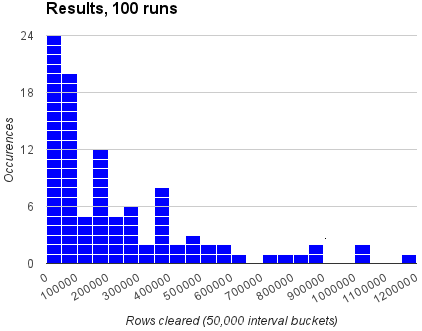
\includegraphics[width=0.5\textwidth]{bucketresults.png}
  \caption{Results from 100 runs.}
  \label{fig:bucketresults}
\end{figure}

The range of results is visualized in figure~\ref{fig:blockresults}, with the median being slightly below 200,000 rows cleared. It also shows that the cluster of results increase in size as the results increase.

\begin{figure}[H]
  \centering
    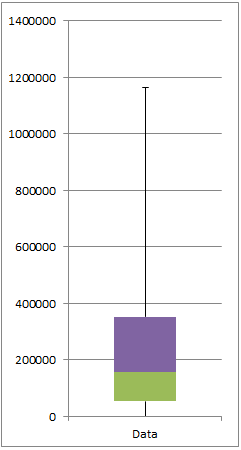
\includegraphics[scale=0.7]{blockresults.png}
  \caption{Block diagram showing the result.}
  \label{fig:blockresults}
\end{figure}

\section{Discussion}
Possible improvements could come from tweaking the genetic algorithm: by modifying the population as well as the cross-over and mutation rates. 

\end{document}


